\section{Praktikum 2}

\subsection{EPK vom Einkaufen}

\begin{figure}[h]
  \caption{EPK vom Einkaufen}
  \label{fig:epk_einkauf}
  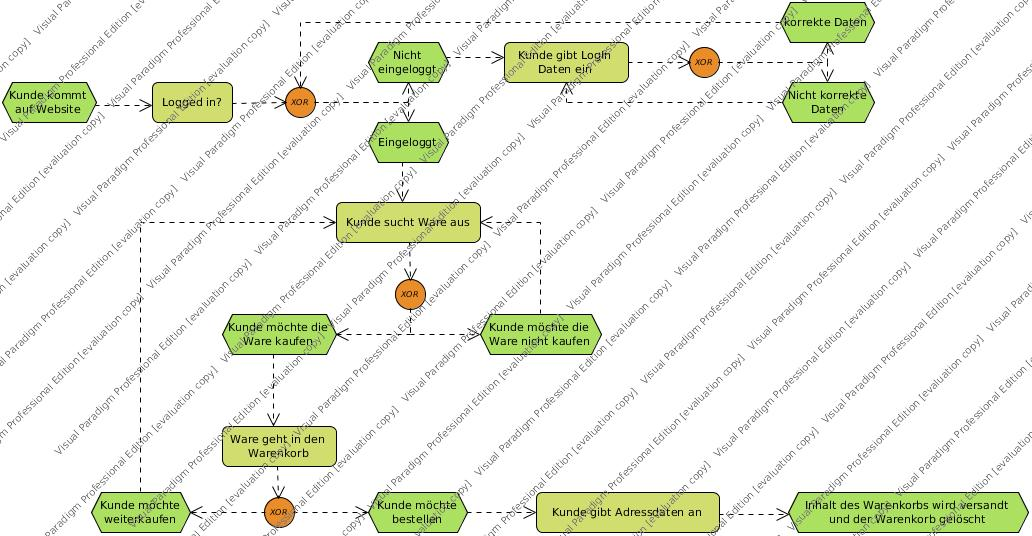
\includegraphics[scale=0.35]{einkaufenEPK}
\end{figure}

\subsection{Vollst\"andiges ER-Modell}
% Einbinden des ERM

\subsection{Erweiterung der Datenbank}
Wie im ersten Praktikum erw\"ahnt, muss man in Rails seine Datenbank nicht ber\"uhren. Wir erzeugten f\"ur die geschachtelte Ware ein weiteres Model namens \texttt{productrelation}. Diese besteht aus zwei Fremdschl\"usseln, welche sich auf \texttt{product} beziehen und aus einem Integer namens \texttt{amount}. Das \texttt{amount} dr\"uckt aus, dass das Superproduct aus \texttt{amount} vielen Subproducts besteht. 

\subsection{Dokumentation 2}

\subsubsection{Geschachtelte Ware}
\texttt{Partials} kann man in Rails als Teilview vermerken. F\"ur h\"aufig auftretende Views kann man sich \texttt{Partials} anlegen und diese dann in einer vollst\"andigen View zusammenwerfen. Zudem kann man auch Argumente \"ubergeben. Wir haben \texttt{Partials} erstellt f\"ur die Ausgabe der Quantit\"at von unseren Raumschiffen. Zu finden ist es unter \texttt{app/views/products/\_quatity.html.erb}. 

\subsubsection{Nutzer und Admins}
Die Passwortverwaltung wird dem Gem \texttt{bcrypt} \"uberlassen. Zwischen Admins und normalen Nutzern wird nicht unterschieden. Nutzer sind nur in der Lage einzukaufen, wenn sie sich vorher registrieren und anmelden. Um Sessions zu starten haben wir einen Controller namens \texttt{Session} erstellt. Mittels diesem \"uberpr\"ufen wir ob ein Nutzer eingeloggt ist oder nicht.

\subsubsection{Prim\"arbedarfsanalyse}
Wir sollten zwei Funktionen zur Prim\"arbedarfanalyse schreiben. Das \texttt{gleitende, arithmetische Mittel} und die \texttt{exponentielle Gl\"attung}. Die beiden Implementationen sind unter \texttt{apps/models/product.rb} zu finden. Unsere Implementation der exponentiellen Gl\"attung bezieht sich immer nur auf die Daten, welche im letzten Jahr gesammelt wurden.

\subsubsection{Software Review}
Siehe dazu Anhang.
